\documentclass[]{article} % For LaTeX2e
\usepackage{nips_adapted,times}
\usepackage{hyperref}
\usepackage{url}
\usepackage{graphicx}
\graphicspath{ {./} }
\usepackage{amsmath}
\title{Edge Caching in Dense Networks}


\author{
Rohin Garg\\
160583\\
BTech, IIT Kanpur
}

% The \author macro works with any number of authors. There are two commands
% used to separate the names and addresses of multiple authors: \And and \AND.
%
% Using \And between authors leaves it to \LaTeX{} to determine where to break
% the lines. Using \AND forces a linebreak at that point. So, if \LaTeX{}
% puts 3 of 4 authors names on the first line, and the last on the second
% line, try using \AND instead of \And before the third author name.

\newcommand{\fix}{\marginpar{FIX}}
\newcommand{\new}{\marginpar{NEW}}

\nipsfinalcopy

\begin{document}


\maketitle

\section*{Introduction}
The demand for rich multimedia services over mobile networks has been soaring at a tremendous pace over recent years. The current cellular architecture will not be able to handle the projected growth in mobile traffic data, especially the increase in multimedia streaming.\\\\ 
A Potential solution: Edge Caching\\\\
In order to cope with the mobile data traffic explosion, mobile network operators (MNOs) deploy small cell base stations (SBS) which operate in conjunction with the macrocell base stations (MBS).
\subsection*{Small Cell Networks}
\begin{itemize}
    \item A way to meet unprecedented traffic demands is to deploy SCNs, which provide short-range, low-power, low-cost small base stations.
    \item But they are not able to solve peak traffic demands using the existing reactive networking paradigm: 
\item Users trafic requests must be served urgently as they come or dropped causing outages Also, a large scale deployment of SCNs is not viable due to site acquisition, installation and backhaul costs.

\end{itemize}

\subsection*{The Role of Proactive Caching in 5G Wireless Networks}
It involves:
\begin{itemize}
    \item It involves network nodes exploiting users’ context information, anticipate users’ demands and use predictive abilities to save resources and cache potential future requests. 
    \item Intelligent pre-allocation of resources and effective scheduling of user requests.
    \item Leveraging the powerful processing capabilities and large memory storage of devices enables network operators to proactively serve predictable peak-hour requests during off-peak times.
    \item Minimization of Inter-ISP traffic
    \item Minimization of Intra-ISP traffic
    \item Minimization of content access delay for users

\end{itemize}

A Model discussed by “Cache in the Air:Exploiting Content Caching and Delivery Techniques for 5G Systems”:
\begin{figure}[!h]
    \centering
    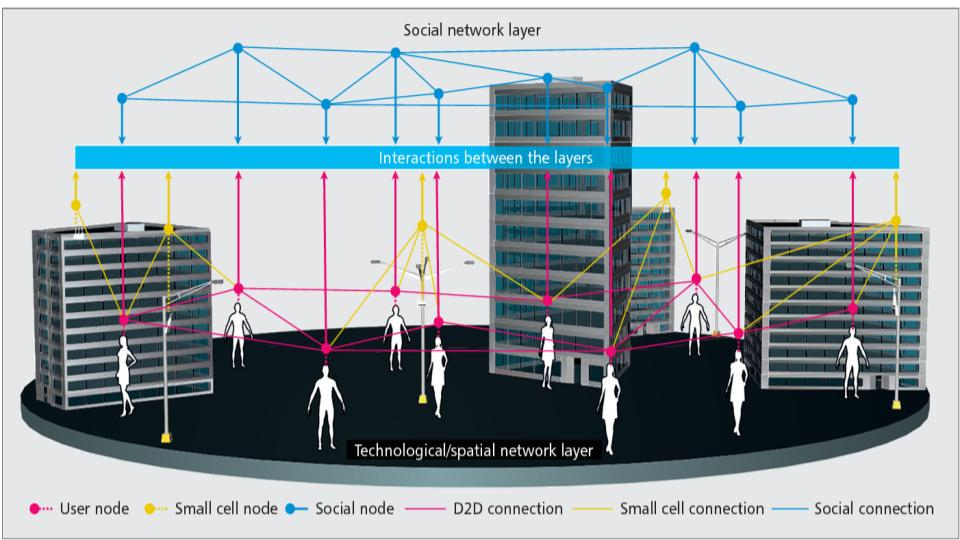
\includegraphics[scale=0.45]{EdgeCaching.jpg}
    \caption{An illustration of an overlay of socially interconnected and spatial network [1]}
\end{figure}
\section*{Problem at Hand}

To analyze the effect of network densification on edge caching performance for different for different caching methods, by:
\begin{itemize}
    \item Conducting experiments on a simple topology, to verify data given in existing literature.
    \item implementing realistic content request patterns.
    \item Creating new network model, dense, and running experiments on it. 
\end{itemize}
I wanted to see the results of existing algorithms on different social scenarios. 
\subsection*{Metrics}
I have some metrics based on which I can calculate the efficiency of the design:
\begin{itemize}
    \item Satisfied requests.
\item Requests routed to MBC and ISP: should be minimized.
\item Hit Rate
\item  Delay in retrieving user requested content
\item Backhaul Load
\end{itemize}

\section*{Experiment 1}

Used a simple network topology to generate data regarding \textit{Hit-Rate} at any cache unit (not necessarily the first one hit), by varying total cache size and SCN cache size. This is \textit{not} a dense network.\\

Topology used:

Various Parameters that had to be decided 
\begin{itemise}
\item Total Content size was fixed.
\item Constant upper limit on individual object size.
\item Cache size in Small Cell was set much lower than Core cache size.
\item Some files were treated much more popular than most others, some not as much, and some were requested rarely.
\item Transmission capacity of each small cell was kept same.
\end{itemise}

\subsection*{Observations}

Ht rate v/s Total cache size.\\

Image

The decreasing slope can be explained as increasing the cache size will only result in caching contents tht are not popular/retrieved only once. They do not contribute to hit-rate.  

\subsection*{Limitations}
\begin{itemise}
\item Not a very realistic case
\item Small cells were not able to communicate properly among themselves.
\item Issue of redundancy of cache: in Core and Small Cells
\item 1 User only contacted 1 Small cell.
\item File popularity was constant; needs to change dynamically, and so do the cached files
\end{itemise}

\section*{Realistic Request Patterns}





\end{document}
